\documentclass[12pt]{scrartcl}
\usepackage[german]{babel}
\usepackage{graphicx}
\usepackage[latin1]{inputenc}
\usepackage[T1]{fontenc}

\usepackage{color}
\usepackage[linkcolor=black, urlcolor=black, citecolor=dblue,
breaklinks, bookmarks, colorlinks]{hyperref}

\begin {document}

\hspace{-0.4cm}\huge \textbf{Freeze Me! - Dokumentation}\vspace{3pt}\\\Large A Media Processing Project \vspace{14pt}\large 

\noindent
\textbf{Stand:} 28.02.2023 \\

\vspace{3pt} \normalsize Gruppe: 
Jan Rekemeyer, Iskander Yusupov und Hendrik Finke

\section{Motivation}
Da das Ziel des Projekts darin bestand, ein Softwareprodukt zu erstellen, entschied sich die Gruppe, eine Motivation im Marketingformat zu erstellen.\\Gl\"uckliche Momente lassen sich in einem Foto festhalten, das dann verschenkt werden kann. Aber was tun mit den gl\"ucklichen Momenten, die auf Video festgehalten wurden? Mit diesem Ansatz suchte die Gruppe nach M\"oglichkeiten, ein Video so in Form eines Bildes festzuhalten, dass dieses sp\"ater beispielsweise als gerahmtes Geschenk pr\"asentiert werden k\"onnte.
Eine weitere Inspiration f\"ur unsere Gruppe waren Videos mit viel Dynamik. Sport, Tanz, aber auch Tiktok-Challenges enthalten viel Bewegung. Beim Fotografieren von sich bewegenden Objekten erzeugt die Einstellung einer Langzeitbeleuchtung den Effekt einer \glqq eingefrorenen\grqq  Bewegung. Diese Fotos haben ihre eigene \"Asthetik und unsere Gruppe wollte versuchen, diesen Effekt mit den im Modul erlernten F\"ahigkeiten zu reproduzieren.

\section{Zielsetzung}Unser Projekt haben wir der folgende Zielsetzung gewidmet: \\
\textit{Wir entwickeln ein Programm, welches es erm\"oglicht aus einem Video ein Bild zu erzeugen, welches die Bewegungsdynamik des Videos \"asthetisch einfasst und dabei den Eindruck fortw\"ahrender Bewegung erh\"alt.}

\section{Langzeitbelichtung - Inspirationsquelle} %Erstmal Hendriks Sektion
\subsection{Motivation}Das in den Er\"offnungsfolien gezeigte Bildmaterial erinnerte uns in Teilen doch recht stark an eine klassische
Langzeitbelichtung, wie
man sie aus der Analogfotografie oder der Fotographie mit DSLRs oder DSLMs kennt. Daher stellten wir uns die Frage, wie man dieses Konzept digital nachtr\"aglich unter Zuhilfenahme eines Videos anstelle eines Fotos reproduzieren kann.\\
 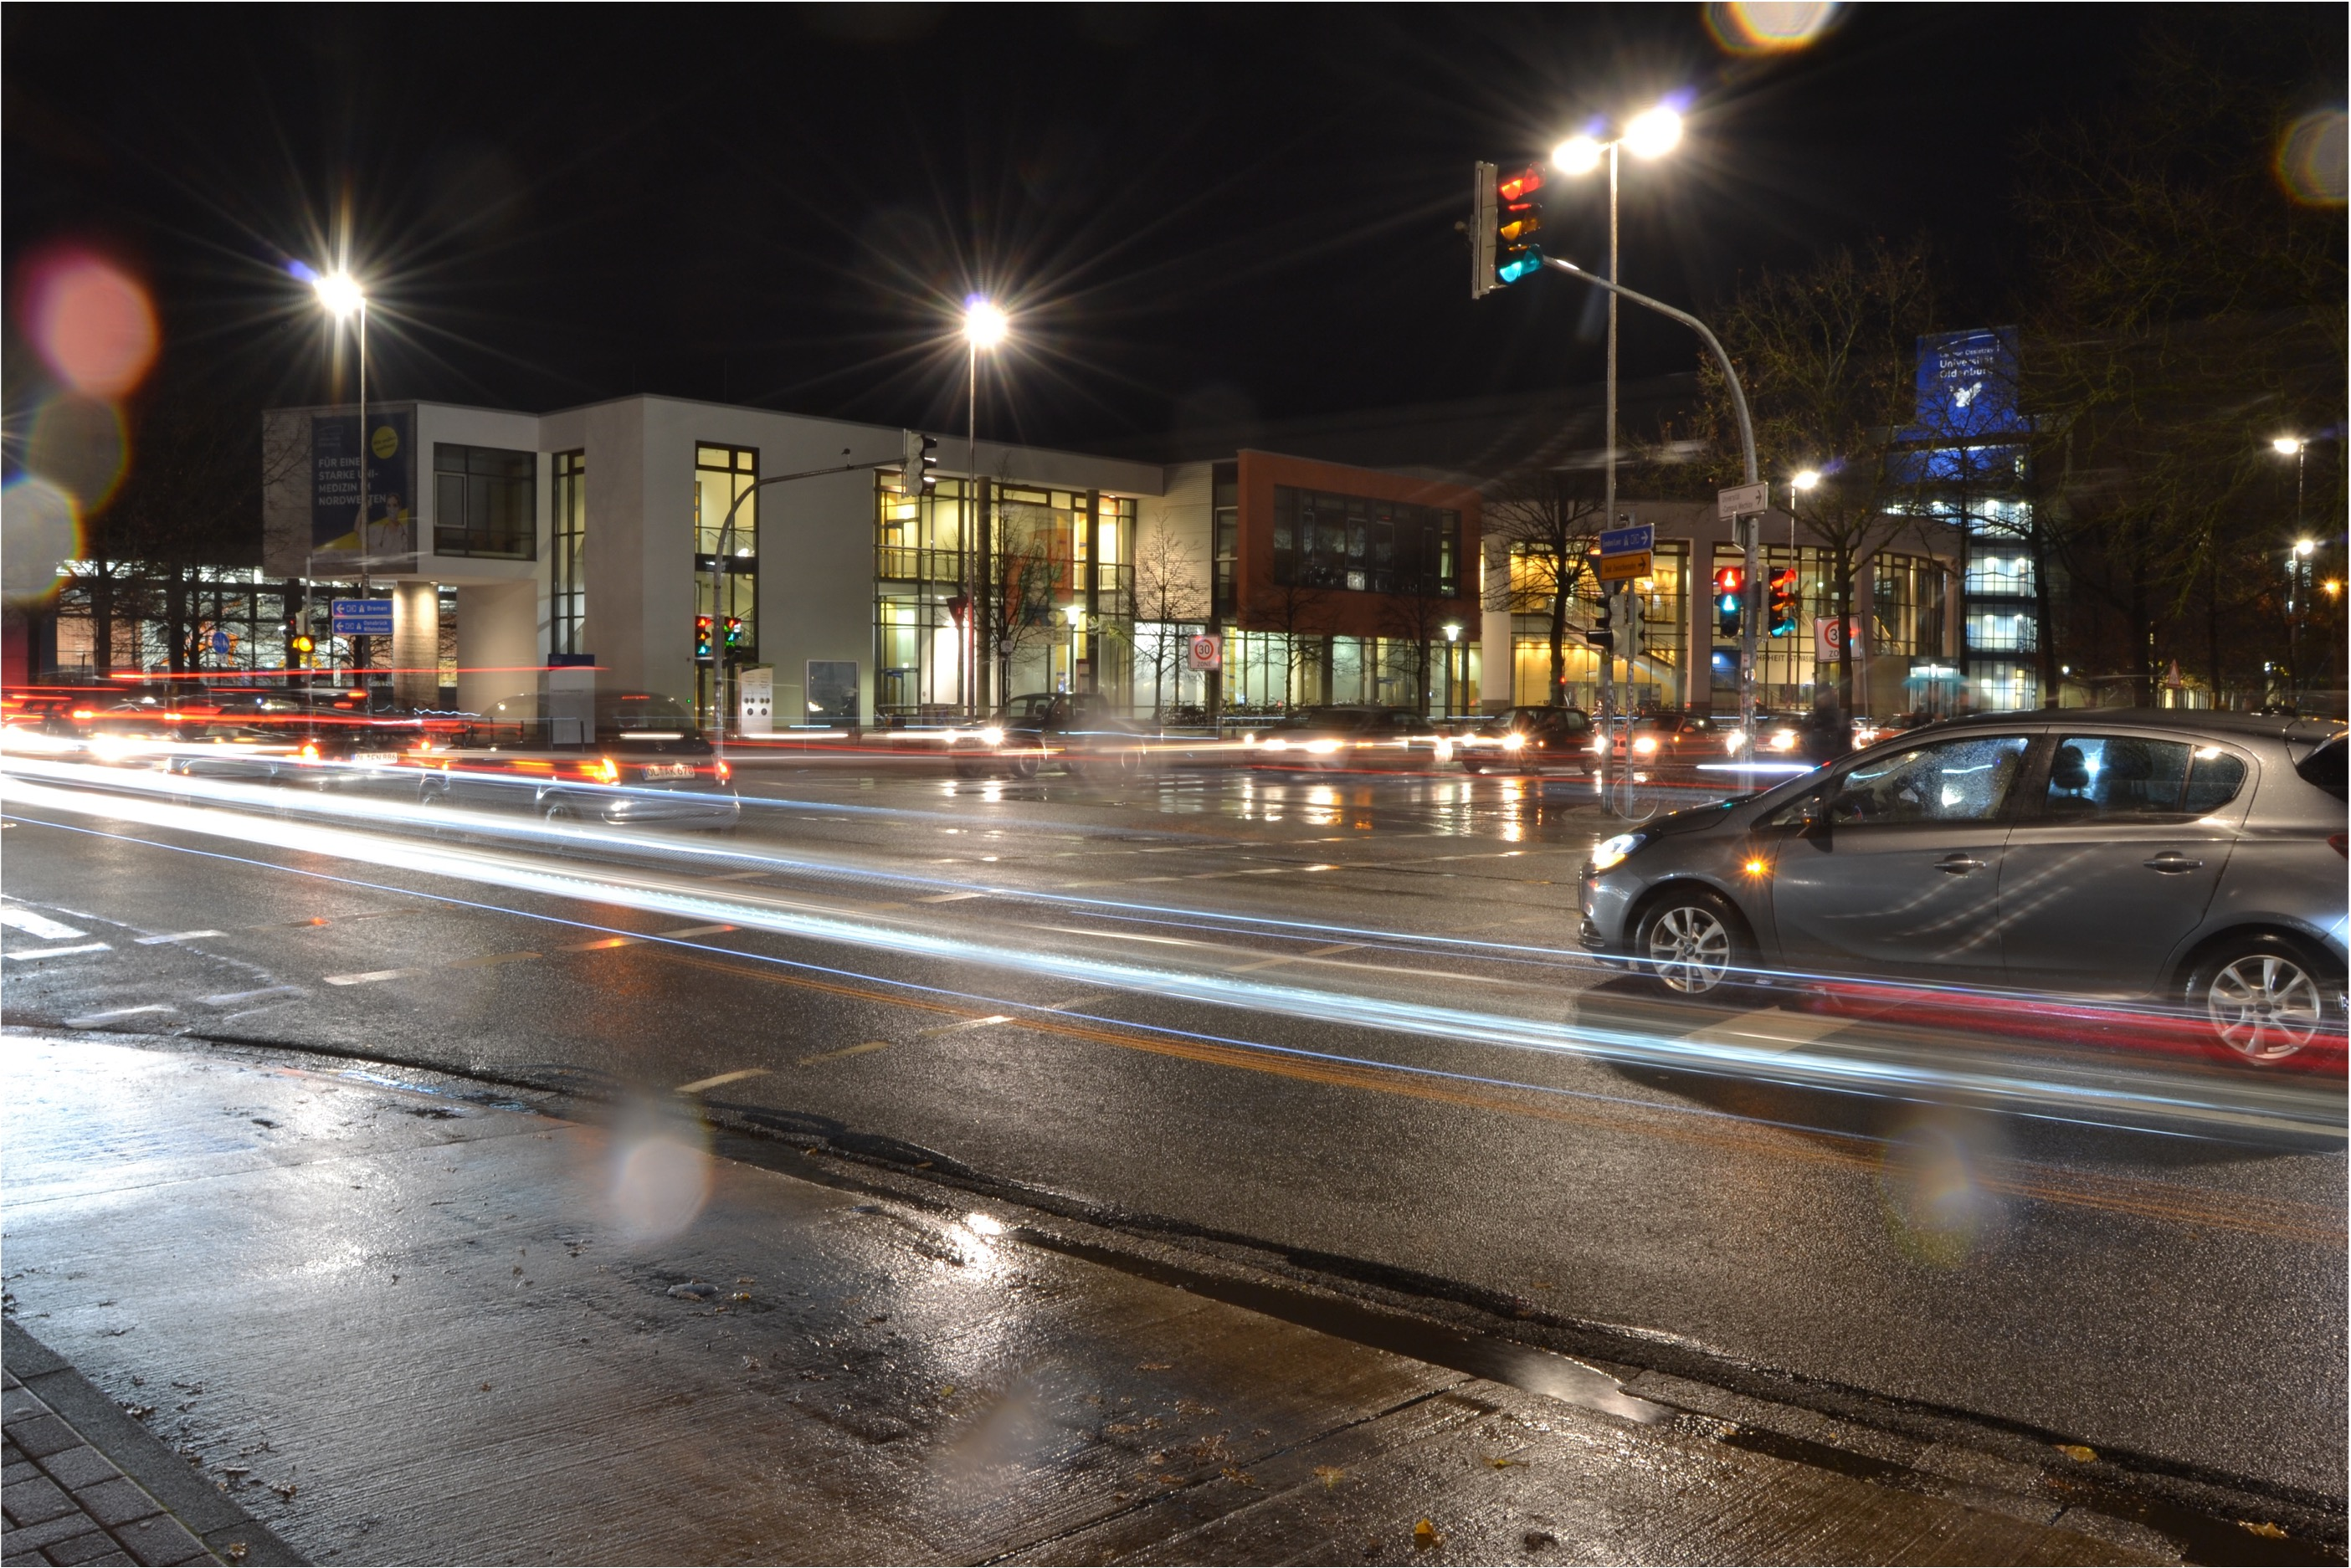
\includegraphics[width=\textwidth]{media/lzb}\\
\subsection{Funktionsweise}Der Ansatz, den wir hierbei Verfolgt haben ist relativ trivial. \"Ahnlich wie klassiche Filter den
Inhaltswert eines Pixels anhand einer ggf. faktorisierten Durchschnittsberechnung mit den umliegenden Pixeln berechnet tun wir ebendieses - jedoch mit den Pixeln gleicher Koordinaten auf anderen Videoframes. Zu diesem Zwecke werden Videos Frame f\"ur Frame betrachtet und dann Pixel f\"ur Pixel in ihre jeweiligen 3 Farbkomponenten zerlegt. Im folgenden wird der Durchschnittswert der Farbwerte errechnet und somit eine Art Langzeitpixel erzeugt, deren Summe das k\"unstlich Langzeitbelichtete Bild ergibt.\\
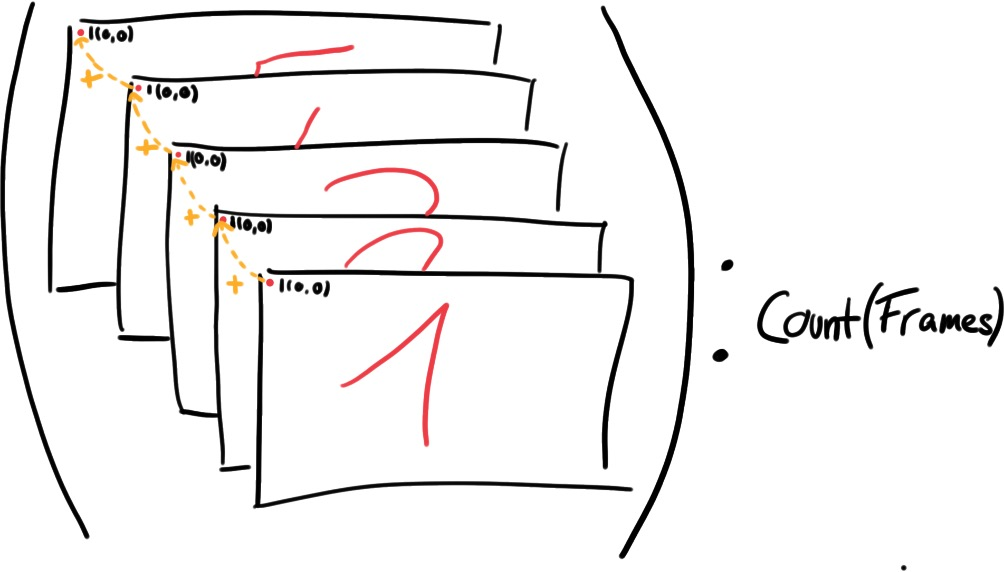
\includegraphics[width=0.6\textwidth]{media/funclzb}
 \subsection{Resultate}Die Resultate waren abh\"angig vom eingegebenen Video durchaus vielversprechend. Ein von uns anf\"anglich eigens erstelltes Video von der Kreuzung der Ammerl\"ander Heerstra{\ss}e mit dem Uhlhornsweg resultierte in einem mehr oder minder matschigen Bild. Das Ergebnis des Contemporary Dancers hingegen war schon erstaunlich dicht an den Hintergrunderscheinungen der Fotos in den Veranstaltungsfolien. Auch das TikTok Video mit dem Sprung resultierte in einem relativ ansehnlichen Ergebnis. Da dieser Ansatz somit der erste nennenswerte Schritt in die Richtung des Gesamtzieles war wurde er beibehalten und die Langzeitbelichtung wurde somit Grundkomponente unseres Projektes.\\
 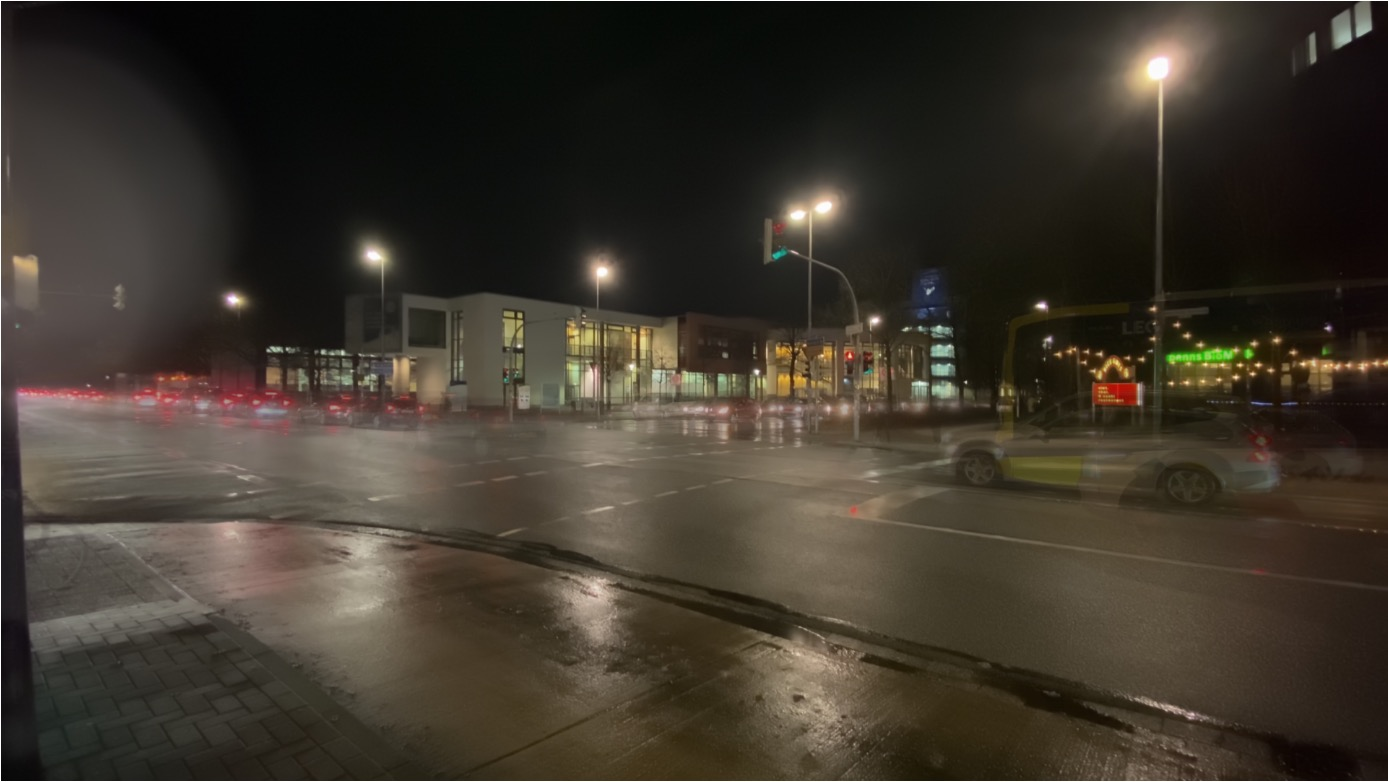
\includegraphics[width=\textwidth]{media/artlzb}
% Anforderungsanalyse

% Langzeitbelichtung
% -> Motivation, Theorie, Codebeschreibung, Resultate
% Grabcut mit Thresholding
% -> Motivation, Theorie, Codebeschreibung, Resultate
% Canny-Edge Detection

\section{Edge Detection und Background Subtraction}
\subsection{Motivation}
Nachdem es der Gruppe gelungen war, Bilder mit einer k\"unstlichen Langzeitblichtung aus dem Video zu erstellen, fiel ein Merkmal auf. Wurde das Video ohne Stativ oder jegliche Art von Unterst\"utzung gedreht, dann führte das leichte Wackeln der Kamera irgendwann dazu, dass sich auch stabile Objekte im Ausgabebild als unscharf herausstellten. Um dieses Merkmal oder Problem zu l\"osen, wurde entschieden, Canny Edge Detection zu verwenden.
Die Idee, der Algorithmus zu verwenden, wurde experimentell geboren. Wir haben versucht, Canny Edge Detection auf ein bereits bearbeitetes Bild anzuwenden. Die Methode erkannte nur Objekte als Kanten, die auf dem Video stabil waren. Dann entschied die Gruppe, dass es m\"oglich ist, Sch\"arfungsverfahren (z. B. einen Laplace-Filter) auf die Pixelkoordinaten mit stabilen Objekten anzuwenden, die mithilfe des Canny Edge Detection auf dem Ausgabebild erhalten werden.
\subsection{Theorie}
Der Canny Edge Detection ist ein mehrstufiger Algorithmus zum Erkennen von Kanten in einem Bild. Der Algorithmus besteht aus vier Stufen. In der ersten Stufe ist es notwendig, Rauschen aus dem Originalbild zu entfernen, f\"ur diese Aufgabe wird der Gau{\ss} Filter angewendet. Der zweite Stufe besteht darin, den Gr\"o{\ss}e entlang der x- und y-Dimension zu erhalten. Dazu wird die Ableitung des Gau{\ss}-Filters berechnet, um dann das Gradient der Bildpixel zu berechnen.
Der Algorithmus geht alle Punkte der Gradientenintensit\"atsmatrix durch und findet die Pixel mit dem maximalen Wert in den Kantenrichtungen.
Das Betrachten der Gruppe von Nachbarn f\"ur jede Kurve in einer Richtung senkrecht zu der gegebenen Kante unterdr\"uckt nicht maximalen Kantenbeitragspixelpunkte. Schlie{\ss}lich wird das Hysterese-Schwellenwertverfahren verwendet, um die Pixel zu bewahren, die h\"oher als die Gradientengr\"o{\ss}e sind, und diejenigen zu vernachl\"assigen, die niedriger als der niedrige Schwellenwert sind.
\subsection{Codebeschreibung}
Zur Optimierung der Ergebnisse wird ein Verfahren zur Bestimmung der Schwellwerte (minVal und maxVal) eingesetzt. Die Schwellwerte werden dann in der OpenCV Methode cv.Canny \"ubergegeben.\\
\subsection{Ergebnis}
Nach dem Ausf\"uhren des Codes ist das erwartete Ergebnis ein Bild mit identifizierten Kanten. Nach Auswertung der Ergebnisse entschied die Gruppe, dass der resultierende Bildsch\"arfungseffekt nicht effektiv genug war, und entschied sich daher, Canny Edge Detection aufzugeben.\\

% MOG2 und KNN
% -> Motivation, Theorie, Codebeschreibung, Resultate

% Frontend: Primer; Paar Buttons eingebaut; Backend mit Funktionen ausgestattet

% Probleme: Coco Dataset,  HED, Django

% Fazit: Limitierungen
% Ausblick: Verbesserungsvorschläge

\section{Edge Detection und Background Subtraction}

\section{Fazit}
\subsection{Limitierungen}
Die Erkennung des Vordergrundes beschr\"ankt die Funktionsweise der Software in Teilen. Von den anf\"anglich 3 angenommenen Testvideos
$ ( $T\"anzer, Kreuzung, TikTok Sprungvideo$ ) $ funktioniert lediglich der T\"anzer wirklich gut. Das Ergebnis des TikTok Sprungvideos ist
ebenfalls durchaus annehmbar, wobei hier das Hinzuf\"ugen eines maskierten Standbildes weitestgehend wertlos ist. Zu diesem Zwecke m\"usste ein Framepicker in der Software implementiert werden. Gleicherma{\ss}en ist der Kontrast der Hintergrundeffekte relativ stark beschr\"ankt, was ein Betrachten der Resultate in schlechten Lichtverh\"altnissen oder gar auf Beamern stark einschr\"ankt. Um diesen Effekt zu verst\"arken h\"atte eine helligkeitsbedingte Faktorisierung genutzt werden k\"onnen, die wir anf\"anglich mal betrachtet haben, deren Notwendigkeit uns im Laufe des Projektes nicht mehr sinnvoll erschien. Retrospektiv w\"are diese Funktion ein sinniges Opt-In gewesen.
\subsection{Ausbaum\"oglichkeiten}
F\"ur eine k\"unftige Ausgestaltung bieten sich die im letzten Block genannten Optionen an: Eine Optimierung des Interfaces um ein Frame zu selektieren, die Option im entsprechenden Frame ein Rechteck zu w\"ahlen, das dann an GrabCut \"ubergeben wird um den Vordergrund zu bestimmen. Dazu w\"are es eine sicherlich gute Option gewesen die Lichtst\"arke in die Langzeitbelichtung einflie{\ss}en zu lassen, um den Kontrast der Schlieren im Hintergrund zu steigern. Darüber hinaus blieben sicherlich noch Optimierungen an der GUI und der Effizienz und damit der Performanz des Systems.
\subsection{Resumee}
Das letztendliche Ergebnis unserer Arbeit entspricht unser Meinung nach dem urspr\"unglichen Ziel - aufgrund der Subjektivit\"at der
\"Asthetik aber l\"asst sich dieses Urteil wohl kaum objektiv f\"allen. Mit der Anwendung der Langzeitbelichtung fand sich f\"ur uns relativ
fr\"uh eine M\"oglichkeit, einen Hintergrund mit den verwaschenen bzw. verschwommenen Hintergrundartefakten zu erzeugen, durch das Erg\"anzen um ein einzelnes, maskiertes Videoframe ist dabei auch die Charakteristik eines Fotos gewährt.

\end{document}
